\documentclass[12pt]{article}

\usepackage[utf8]{inputenc}
\usepackage[greek,english]{babel}
\usepackage[unicode]{hyperref}
\usepackage{alphabeta}
\usepackage{amsmath}
\usepackage{mathtools}
\newcommand{\Lagr}{\mathcal{L}}
\usepackage{graphicx}
\usepackage{bookmark}
 
\begin{document}

\author{Κωνσταντίνος Λέτρος 8851}

 \begin{titlepage} % Suppresses displaying the page number on the title page and the subsequent page counts as page 1
	\newcommand{\HRule}{\rule{\linewidth}{0.5mm}} % Defines a new command for horizontal lines, change thickness here
	
	\center % Centre everything on the page
	
	%------------------------------------------------
	%	Headings
	%------------------------------------------------
	
	\textsc{\LARGE ΠΟΛΥΤΕΧΝΙΚΗ ΣΧΟΛΗ ΑΠΘ}\\[1.5cm] % Main heading such as the name of your university/college
	
	\textsc{\Large ΤΜΗΜΑ ΗΛΕΚΤΡΟΛΟΓΩΝ ΜΗΧΑΝΙΚΩΝ ΚΑΙ ΜΗΧΑΝΙΚΩΝ ΥΠΟΛΟΓΙΣΤΩΝ}\\[0.5cm] % Major heading such as course name
	
	 
	
	%------------------------------------------------
	%	Title
	%------------------------------------------------
	
	\HRule\\[0.4cm]
	
	{\huge\bfseriesΠροσομοίωση και Μοντελοποίηση Συστημάτων}\\[0.4cm] % Title of your document
	
	\HRule\\[1.5cm]
	
	%------------------------------------------------
	%	Author(s)
	%------------------------------------------------
	{\huge\bfseries Κωνσταντίνος Λέτρος \newline 8851}\\[0.4cm]	
	\vfill	
	{\huge\bfseries Εργασία 1}\\[0.4cm]  % Title of your document
	% If you don't want a supervisor, uncomment the two lines below and comment the code above
	%{\large\textit{Author}}\\
	%John \textsc{Smith} % Your name
	
	%------------------------------------------------
	%	Date
	%------------------------------------------------
	
	\vfill\vfill\vfill % Position the date 3/4 down the remaining page
	
	{\large\today} % Date, change the \today to a set date if you want to be precise
	
	%------------------------------------------------
	%	Logo
	%------------------------------------------------
	
	%\vfill\vfill
	%\includegraphics[width=0.2\textwidth]{placeholder.jpg}\\[1cm] % Include a department/university logo - this will require the graphicx package
	 
	%----------------------------------------------------------------------------------------
	
	\vfill % Push the date up 1/4 of the remaining page
	
\end{titlepage}





\newpage
\section{Θέμα 1 }
\subsection{Θεωρητική Ανάλυση}
Δίνεται το σύστημα μάζας-ελατηρίου-αποσβεστήρα που φαίνεται στο Σχήμα 1, όπου $b$ είναι η σταθερά απόσβεσης, $k$ η σταθερά του ελατηρίου, $u(t)$ μια εξωτερική δύναμη (είσοδος του συστήματος) και $y(t)$ είναι η μετατόπιση της μάζας  $m$ εξαιτίας της δύναμης που εφαρμόζεται πάνω της (έξοδος του συστήματος).
\\ \\
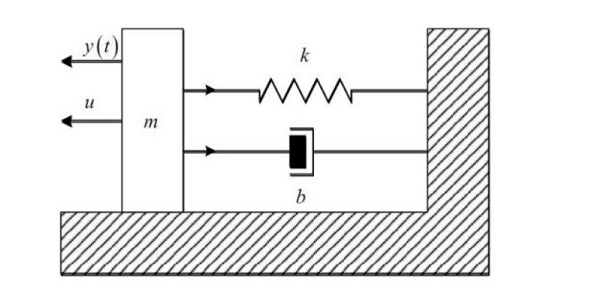
\includegraphics[width=\linewidth]{sys1.jpg}
\centerline{Σχήμα 1: Σύστημα μάζας, ελατηρίου, αποσβεστήρα}
\newline
\newline
\newline
α) Για να βρούμε το μαθηματικό μοντέλο που περιγράφει τη δυναμική συμπεριφορά του συστήματος εφαρμόζουμε το θεμελιώδη νόμο της μηχανικής (Δεύτερος Νόμος του Νεύτωνα):
\newline
\newline
$m \ddot{y}=u-ky-b\dot{y} \Rightarrow  \ddot{y}=-\frac{b}{m}\dot{y}-\frac{k}{m}y+\frac{1}{m}u \quad \left(1\right)$
\newline
\newline
όπου οι αρχικές συνθήκες είναι μηδενικές από υπόθεση, \quad $y(0)=\dot{y}(0)=0$
\newline
\newline
Μπορούμε να γράψουμε τη διαφορική εξίσωση $\left(1\right)$  με τη μορφή \quad $\ddot{y}=\theta^{*T}\Delta$ \quad όπου
\newline
\newline
$\theta_{1}^{*}=
\begin{bmatrix}
		\frac{β}{m} & \frac{k}{m}
\end{bmatrix}^{T}$
\qquad
$\theta_{2}^{*}=
\begin{bmatrix}
		\frac{1}{m}
\end{bmatrix}^{T}$
\qquad
$\theta^{*}=
\begin{bmatrix}
		\theta_{1}^{*T} & \theta_{2}^{*T}
\end{bmatrix}^{T}=
\begin{bmatrix}
		\frac{β}{m} & \frac{k}{m} & \frac{1}{m}
\end{bmatrix}^{T}$
\newline 
\newline 
και \quad
$\Delta=
\begin{bmatrix}
		-\dot{y} & -y & u
\end{bmatrix}^{T}
 \quad$ ή $ \quad \Delta(s)=
\begin{bmatrix}
		-sY(s) & -Y(s) & U(s)
\end{bmatrix}^{T} \quad (*)$ 
\newline
\newline
\newline
Ωστόσο, δεν γνωρίζουμε-μετράμε τις τιμές για την πρώτη και δεύτερη παράγωγο του $y(t)$, οπότε για να μπορέσουμε να προχωρήσουμε θεωρούμε ευσταθές πολυώνυμο $\Lambda(s)$  (όλες του οι ρίζες ανήκουν στο αριστερό μιγαδικό ημιεπίπεδο) στο πεδίο $Laplace$ δευτέρου βαθμού, \quad $\Lambda(s)=s^{2}+\lambda_{1}s+\lambda_{2}$ \quad και \quad $\lambda=
\begin{bmatrix}
		\lambda_{1} & \lambda_{2}
\end{bmatrix}^{T} \quad$ όπου $\lambda_{1},\lambda_{2}>0$
ώστε με τη χρήση του όρου $1/\Lambda(s)$ να φιλτράρουμε την έξοδο.
\newline
\newline
Έτσι, το σύστημα μπορεί να παραμετροποιηθεί γραμμικά και να γραφτεί στη μορφή γραμμικής οπισθοδρόμησης \quad  $y=\theta^{T}_{\lambda}\zeta$ \quad  στο πεδίο του χρόνου ή στο πεδίο $Laplace$ ως \quad $Y(s)=\theta^{T}_{\lambda}\zeta(s)$ \quad όπου $\zeta$ το διάνυσμα οπισθοδρόμησης.
\newline
\newline 
 $\theta_{\lambda}=\begin{bmatrix}
		\theta_{1}^{*T}-\lambda^{T} \quad& \theta_{2}^{*T}
\end{bmatrix}^{T}=
\begin{bmatrix}
		\frac{β}{m}-\lambda_{1} \quad &  \frac{k}{m}-\lambda_{2} \quad &  \frac{1}{m}
\end{bmatrix}^{T}
$
\newline
\newline
και
\newline
\newline
$
\zeta(s)=\begin{bmatrix}
		-\frac{\Delta^{T}(s)Y(s)}{\Lambda(s)} & \frac{\Delta^{T}(s)U(s)}{\Lambda(s)}
\end{bmatrix}^{T}\Rightarrow
\zeta(s)=\begin{bmatrix}
		-\frac{sY(s)}{s^{2}+\lambda_{1}s+\lambda_{2}} \quad &  -\frac{Y(s)}{s^{2}+\lambda_{1}s+\lambda_{2}} \quad &  \frac{U(s)}{s^{2}+\lambda_{1}s+\lambda_{2}}
\end{bmatrix}^{T}$
\newline
\newline
\newline
\newline
Επομένως \quad $Y(s)=
\begin{bmatrix}
		\frac{β}{m}-\lambda_{1} \quad &  \frac{k}{m}-\lambda_{2} \quad &  \frac{1}{m}
\end{bmatrix}
\begin{bmatrix}
		-\frac{sY(s)}{s^{2}+\lambda_{1}s+\lambda_{2}} \quad &  -\frac{Y(s)}{s^{2}+\lambda_{1}s+\lambda_{2}} \quad &  \frac{U(s)}{s^{2}+\lambda_{1}s+\lambda_{2}}
\end{bmatrix}^{T}  \quad (*)$ 
\newline
\newline
και επιστρέφοντας στο πεδίο του χρόνου\quad $y(t)=\Lagr^{-1}(Y(s))$ 
\newline
\newline
$(*)$ όπου με $\Lagr(f(t))$ συμβολίζεται ο μετασχηματισμός $Laplace$ της $f(t)$ και
\newline
$\quad Y(s)= \Lagr(y(t)) \quad U(s)= \Lagr(u(t)) \quad \Delta(s)= \Lagr(\Delta) \quad \zeta= \Lagr^{-1}(\zeta(s))$
\newline
\newline
\newline
\newline
β)\quadΣτη συνέχεια θα χρησιμοποιήσουμε τη μέθοδο ελαχίστων τετραγώνων με στόχο να ελαχιστοποιήσουμε το σφάλμα εκτίμησης και τελικά να εκτιμήσουμε με σχετική ακρίβεια τις επιθυμητές παραμέτρους. Για το σκοπό αυτό θεωρούμε, αρχικά, τη συνάρτηση σφάλματος $e(\theta,\hat{\theta})$.
\\
\[e(\theta,\hat{\theta})=y-\hat{y}=y-\hat{\theta}^{T}_{\lambda}\phi\]
\\
 όπου με $\hat{\theta}$ και $\hat{y}$ συμβολίζονται οι εκτιμήσεις των $\theta$ και $y$ αντίστοιχα και $\phi$ ο πίνακας που περιέχει τις αριθμητικές τιμές του διανύσματος οπισθοδρόμησης $\zeta$.
\\ \\
Έπειτα επιδιώκουμε να ελαχιστοποιήσουμε την $l(\theta,\hat{\theta})=\frac{1}{2}ee^{T}$ , η οποία είναι κυρτή συνάρτηση (έχει μοναδική ελάχιστη τιμή) ως προς $\hat{\theta}$.
Για να έχουμε την ελάχιστη τιμή \quad $min_{\hat{\theta}} l(\theta,\hat{\theta})$ λύνουμε την εξίσωση
\\ 
\[ \frac{ \partial l}{\partial \hat{\theta}}\Bigr|_{\substack{\hat{\theta} =\theta_{0}}}=0 \]
 \\
 από όπου προκύπτει 
 \[
 \phi\phi^{T}\theta_{0}=\phi y
\] 
 \\ 
και τέλος λύνουμε το παραπάνω σύστημα για να βρούμε το $\theta_{0}$. Όταν ελαχιστοποιείται το σφάλμα, έχουμε
 \\
\[ e(\theta,\hat{\theta})\approx 0 \Rightarrow y-\hat{y} \approx 0 \Rightarrow (\theta^{T}_{\lambda}-\hat{\theta}^{T}_{\lambda})\phi \approx 0\] 
και αν ο πίνακας $\phi$ είναι αντιστρέψιμος
\[\theta^{T}_{\lambda} \approx \theta_{0} \Rightarrow\]
 
 \[ \theta_{0} \approx
 \begin{bmatrix}
		\frac{β}{m}-\lambda_{1} \quad &  \frac{k}{m}-\lambda_{2} \quad &  \frac{1}{m}
\end{bmatrix}^{T}\]
 \\
 Τέλος, λύνοντας την παραπάνω εξίσωση βρίσκουμε τις εκτιμήσεις των άγνωστων παραμέτρων.
\\
\\
\\
\\
γ) Η ανάλυση που έγινε προηγουμένως, χρησιμοποιήθηκε για τη δημιουργία ενός αλγορίθμου σε περιβάλλον $Matlab$ που έχει ως στόχο την εκτίμηση των παραμέτρων $m = 15kg$, $b = 0,2kg/sec$ και $k = 2kg/sec^2$ για γνωστή είσοδο $u(t) = 5 sin(2t) + 10.5 \quad(N)$.
\\
\\
Αρχικά επιλύουμε αριθμητικά τη διαφορική εξίσωση $(1)$ για τις παραπάνω \\ παραμέτρους και δημιουργούμε έναν πίνακα τιμών-δεδομένων για την είσοδο $u(t)$ και την έξοδο $y(t)$ με τιμές από $t=0$  μέχρι $t=10 sec$ με βήμα $0,1$ όπως φαίνεται παρακάτω.
\\
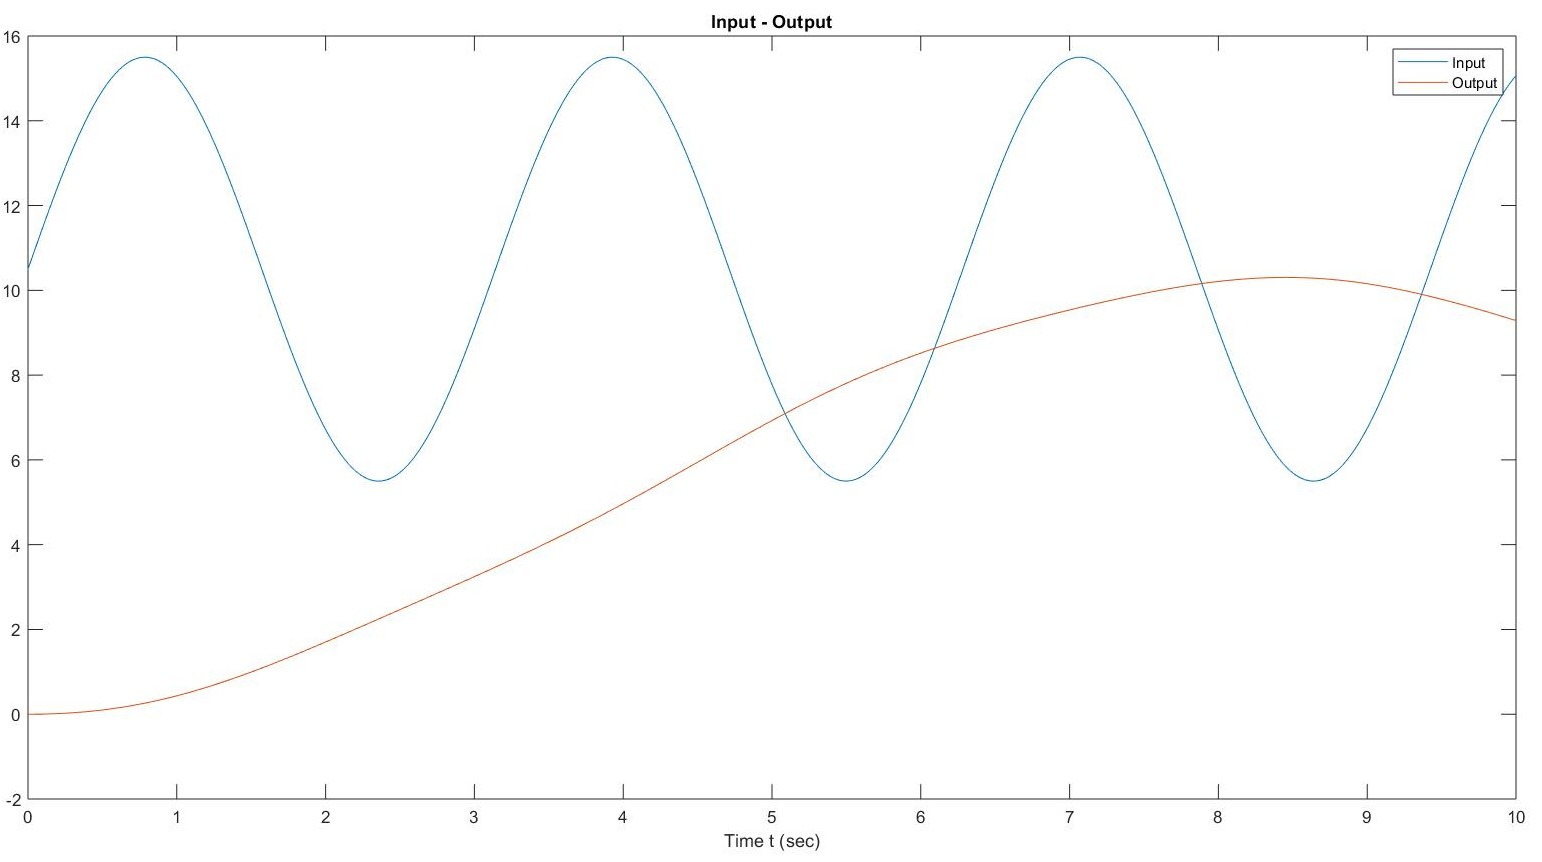
\includegraphics[width=\linewidth]{sys1_inp_out.jpg}
\centerline{Σχήμα 2: Είσοδος - Έξοδος Συστήματος}
\newline
\newline
\newline
Στη συνέχεια ακολουθούμε τα βήματα της ανάλυσης, κατασκευάζουμε το διάνυσμα οπισθοδρόμησης ώστε να παραμετροποιήσουμε γραμμικά το σύστημα και εφαρμόζουμε τη μέθοδο ελαχίστων τετραγώνων για να ελαχιστοποιήσουμε το σφάλμα.
\\
\\Το φίλτρο που χρησιμοποιήθηκε κατά την εκτέλεση του κώδικα στο $Matlab$ επιλέχθηκε αρχικά σχετικά τυχαία (σε λογικές τιμές - εξηγείται παρακάτω) ως $\Lambda(s)=s^{2}+3s+2$, από όπου προέκυψαν αρχικά οι τιμές $\frac{1}{\hat{m}} = 0,066492 kg^{-1}$, $\frac{\hat{b}}{\hat{m}} = 0,13307\quad sec^{-1}$, $\frac{\hat{k}}{\hat{m}} = 0,012686 \quad sec^{-2}$ . Στη συνέχεια το φίλτρο αναπροσαρμόστηκε και πήρε την τελική του μορφή, $\Lambda(s)=s^{2}+0.13s+0.013$ 
δηλαδή $\lambda_{1}=0,13$ και $\lambda_{2}=0,013$. Αποδείκνύεται $(**)$ ότι το φίλτρο που θα δώσει καλύτερες εκτιμήσεις είναι εκείνο για το οποίο ισχύει $\theta_{1}^{*}-\lambda=0$. Επομένως, βρίσκουμε μια πρώτη εκτίμηση των παραμέτρων για κάποιο τυχαίο φίλτρο, που τα κέρδη του έχουν τιμές λογικές, δηλαδή θα πρέπει να προσεγγίζουν ένα λόγο σταθεράς απόσβεσης ή σταθεράς ελατηρίου προς μάζα. Στη συνέχεια θέτουμε τους λόγους $\frac{\hat{b}}{\hat{m}} = 0,13307 \quad sec^{-1}$, $\frac{\hat{k}}{\hat{m}} = 0,012686 \quad sec^{-2}$ (προσεγγιστικά εδώ) ως τα νέα κέρδη του φίλτρου και παίρνουμε τελικά καλύτερα αποτελέσματα, με μικρότερο σφάλμα. Συνεχίζοντας επαναληπτικά την παραπάνω διαδικασία, μπορουμέ να πετύχουμε πολύ μεγάλη ακρίβεια στις εκτιμήσεις. \\ \\
Πρέπει να σημειωθεί, ωστόσο, ότι τα κέρδη του φίλτρου βρίσκονται κοντά στο φανταστικό άξονα και μικρές διαταραχές στις θέσεις των πόλων θα μπορούσαν να οδηγήσουν το σύστημα σε αστάθεια. Στην περίπτωση αυτή θα πρέπει τα κέρδη, για λόγους καλής λειτουργίας, να ληφθούν μεγαλύτερα.\\ \\
Έτσι, οι εκτιμώμενες τιμές που προκύπτουν τελικά είναι 
\\ \\
$\hat{m} =  14,999732 kg$, $\hat{b} =  0,1994139 kg/sec$, $\hat{k} = 2,0001126 kg/sec^2$
\\ \\
που παρουσιάζουν σφάλμα, το οποίο μπορεί να ελαττωθεί ακόμα περισσότερο, μειώνοντας την τιμή του βήματος.
\\ \\ \\
$(**)$ Θα δείξουμε ότι τα κέρδη $\lambda_{1},\lambda_{2},...,\lambda_{n}$ ενός ευσταθούς φίλτρου $\Lambda(s)$ οδηγούν σε καλύτερες εκτιμήσεις όταν ισχύει η σχέση $\theta_{1}^{*} \approx \lambda$ .
\\
\[ \theta_{1}^{*} - \lambda  \approx 0 \Rightarrow \theta_{1}^{*T}-\lambda^{T} \approx 0 \Rightarrow \theta_{\lambda} \approx [0 \quad \theta_{2}^{*T}]^{T} \]
Επομένως,
\[ \hat{Y}(s) = [0 \quad \theta_{2}^{*T}] \left[ -\frac{\Delta^{T}(s) Y(s)}{\Lambda(s)} \quad \frac{\Delta^{T}(s)U(s)}{\Lambda(s)} \right]^{T} \Rightarrow \hat{Y}(s) = \theta_{2}^{*T} \frac{\Delta^{T}(s)U(s)}{\Lambda(s)} \]
\\ \\
Δηλαδή δεν υπάρχει καθόλου η παρουσία των παραγώγων της εξόδου που είναι άγνωστες και εμφανίζεται μόνο η είσοδος (με τις παραγώγους της) που είναι γνωστή, οπότε τα αποτελέσματά μας δεν αλλοιώνονται από προσεγγίσεις-φιλτράρισμα και είναι πιο ακριβή.
\subsection{Κώδικας και αρχεία στο $Matlab$}

Ο αλγόριθμος που αναπτύχθηκε αποτελείται συνολικά από τρία διακριτά αρχεία, τα $testAlgorithm.m$, $leastSquares.m$ και $regressionVector.m$. Για την εκτέλεση του αλγορίθμου τρέχουμε το αρχείο $testAlgorithm.m$ .
\\ \\
Στο αρχείο $testAlgorithm.m$ δίνονται τα δεδομένα του προβλήματος, επιλύεται η διαφορική εξίσωση $(1)$ για τους λόγους που αναφέρθηκαν και τέλος παράγονται οι εκτιμήσεις των παραμέτρων με τη χρήση της συνάρτησης $leastSquares$.
\\ \\
Στο αρχείο $leastSquares.m$ υλοποιείται η μέθοδος ελαχίστων τετραγώνων όπως αναφέρθηκε στη θεωρητική ανάλυση, ενώ για το διάνυσμα οπισθοδρόμησης καλείται η συνάρτηση $regressionVector$. Για την εύρεση του $\theta_{0}$ από την επίλυση του γραμμικού συστήματος που προέκυψε στο τέλος της μεθόδου, χρησιμοποιήθηκε η συνάρτηση $linsolve$ του $Matlab$.
\\ \\
Τέλος, στο αρχείο $regressionVector.m$ παράγεται το διάνυσμα οπισθοδρόμησης. Συγκεκριμένα, αυτό επιτυγχάνεται, αναλυτικότερα, ως εξής.\\
Γράφουμε το διάνυσμα οπισθοδρόμησης $\zeta(s)$ στο πεδίο $Laplace$ ως
\\
$\zeta(s)=
\begin{bmatrix}
		\zeta_{1}(s) & \zeta_{2}(s) & \zeta_{3}(s)
\end{bmatrix}^{T}$ \quad άρα
\newline
\newline
$\zeta_{1}(s)=-\frac{sY(s)}{s^2+\lambda_{1}s+\lambda_{2}} \Rightarrow \left( s^2+\lambda_{1}s+\lambda_{2} \right)\zeta_{1}(s) = -sY(s)\xRightarrow{I.L.T.}$
\newline
$ \frac{d^2\zeta_{1}}{dt^2} +\lambda_{1}\frac{d\zeta_{1}}{dt}+\lambda_{2}\zeta_{1}=-\frac{dy}{dt} \Rightarrow \ddot{\zeta_{1}}+ \lambda_{1}\dot{\zeta_{1}}+\lambda_{2}\zeta_{1}=-\dot{y}$
\newline
\newline
\newline
$\zeta_{2}(s)=-\frac{Y(s)}{s^2+\lambda_{1}s+\lambda_{2}} \Rightarrow \left( s^2+\lambda_{1}s+\lambda_{2} \right)\zeta_{2}(s) = -Y(s)\xRightarrow{I.L.T.}$
\newline
$ \frac{d^2\zeta_{2}}{dt^2} +\lambda_{1}\frac{d\zeta_{2}}{dt}+\lambda_{2}\zeta_{2}=-y \Rightarrow \ddot{\zeta_{2}} +\lambda_{1}\dot{\zeta_{2}}+\lambda_{2}\zeta_{2}=-y$
\newline
\newline
\newline
$\zeta_{3}(s)=\frac{U(s)}{s^2+\lambda_{1}s+\lambda_{2}} \Rightarrow \left( s^2+\lambda_{1}s+\lambda_{2} \right)\zeta_{3}(s) = U(s)\xRightarrow{I.L.T.}$
\newline
$ \frac{d^2\zeta_{3}}{dt^2} +\lambda_{1}\frac{d\zeta_{3}}{dt}+\lambda_{2}\zeta_{3}=u \Rightarrow \ddot{\zeta_{3}} +\lambda_{1}\dot{\zeta_{3}}+\lambda_{2}\zeta_{3}=u$
\newline
\newline
Με τη βοήθεια της συνάρτησης $lsim$ του $Matlab$ επιλύουμε τις παραπάνω διαφορικές εξισώσεις με μηδενικές αρχικές συνθήκες και βρίσκουμε αριθμητικά στο χρόνο τις $\zeta_{1},\zeta_{2},\zeta_{3}$ με τη μορφή πίνακα για τις τιμές χρόνου από $t_{0}=0$  μέχρι $t=10 sec$ με βήμα $0,1$.
\newline
\newline
Σημείωση: Η επίλυση της διαφορικής εξίσωσης $(1)$ έγινε, επίσης, με χρήση της συνάρτησης $lsim$ για τον ίδιο χρόνο, βήμα και αρχικές συνθήκες.
\subsection{Έλεγχος Σφαλμάτων}
Προκειμένου να ελέγξουμε τις εκτίμησεις μας για τις ζητούμενες παραμέτρους $m,b,k$ θεωρούμε τo σφάλμα
\[ e=|y-\widetilde{y}| \] 
που μας δείχνει πόσο διαφέρει, κατά απολύτη τιμή,  η έξοδος του συστήματος όταν γνωρίζουμε τις παραμέτρους και όταν εκτιμούμε τις παραμέτρους.
\\ \\
Με $\widetilde{y}$ συμβολίζεται η εκίμηση του $y$, όπως προκύπτει από την επίλυση της διαφορικής εξίσωσης (1) για τις τιμές των παραμέτρων μου εκτιμήσαμε.
\\ \\
Η γραφική παράσταση του σφάλματος φαίνεται, στο Σχήμα 3 για $t=0$, έως $t=1500sec$ (ως απόδειξη καλής λειτουργίας του αλγορίθμου) με βήμα $0,1$.
\\
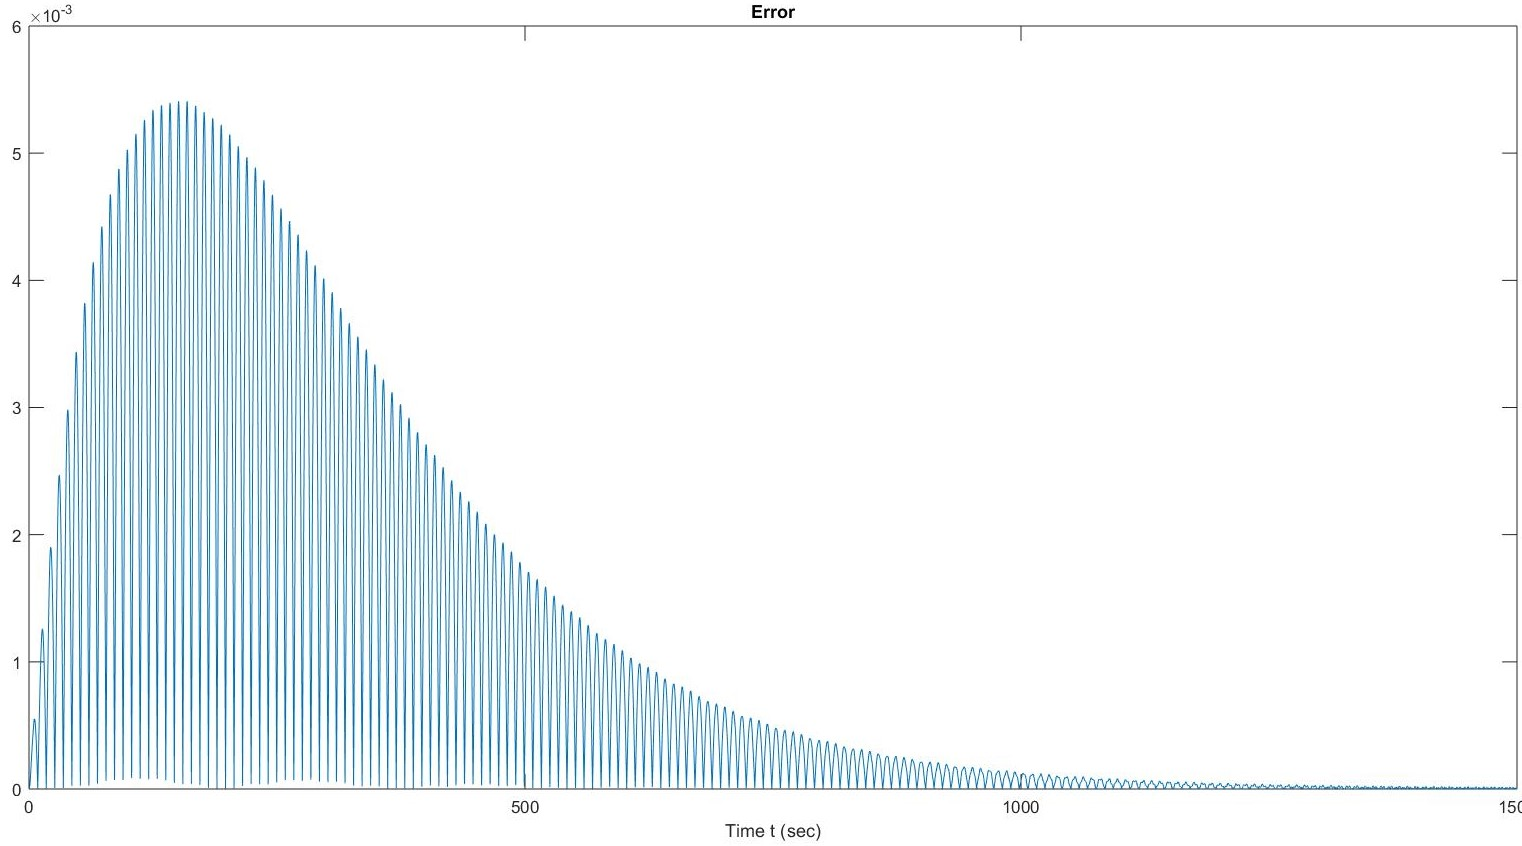
\includegraphics[width=\linewidth]{sys1_error.jpg}
\centerline{Σχήμα 3: Συνάρτηση Σφάλματος $e$}
\newline
\newline
Το σφάλμα είναι της τάξης του $10^{-3}$ στη χειρότερη περίπτωση και μπορεί να ελαττώθει ακόμα περισσότερο όσο μειώνεται το βήμα ή τα κέρδη πλησιάζουν στο $θ_{1}^{*}$.
\newpage
\section{Θέμα 2}
\subsection{Θεωρητική Ανάλυση}
Δίνεται το κύκλωμα που φαίνεται στο Σχήμα 3, όπου $u_{1}(t)=2sin(t) \quad V$, \\$ u_{2}(t)=1 V$ πηγές τάσεις (γνωστές είσοδοι του συστήματος) και $V_{R}(t),V_{C}(t)$ οι τάσεις στα άκρα της αντίστασης $R$, και του πυκνωτή $C$, αντίστοιχα (έξοδοι του συστήματος).
\\ \\
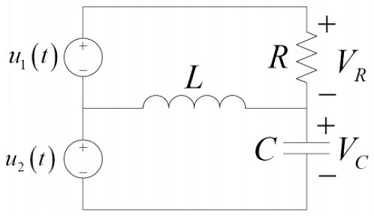
\includegraphics[width=\linewidth]{sys2.jpg}
\centerline{Σχήμα 4: Σύστημα - Κύκλωμα $RLC$}
\newline
\newline
α) Για να εκτιμήσουμε τον πίνακα μεταφοράς του συστήματος θα χρειαστεί αρχικά να βρούμε το μαθηματικό μοντέλο που περιγράφει τη δυναμική συμπεριφορά του και να γράψουμε το σύστημα στη μορφή εξισώσεων κατάστασης. Εφαρμόζουμε, λοιπόν, το νόμο τάσεων του $Kirchhoff$ όταν τα ρεύματα των βρόχων είναι $i_{1}(t),i_{2}(t)$, όπως φαίνονται στο Σχήμα 5.
\\ \\
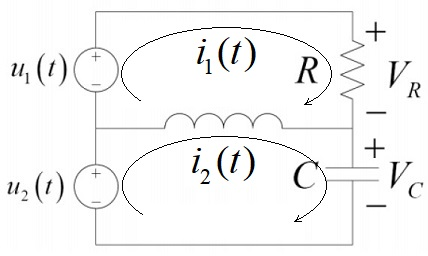
\includegraphics[width=\linewidth]{sys2_2.jpg}
\centerline{Σχήμα 5: Σύστημα - Κύκλωμα $RLC$}
\newline
\newline
\[
   \left\{
                \begin{array}{ll}
                  u_{1}(t)=V_{R}(t)+L\left(\frac{di_{1}(t)}{dt}-\frac{di_{2}(t)}{dt}\right)\qquad(1)\\
                  u_{2}(t)=L\left(\frac{di_{2}(t)}{dt}-\frac{di_{1}(t)}{dt}\right)+V_{C}(t)  \qquad(2)
                \end{array}
              \right.
\]
Επίσης έχουμε: \\ \\
$
   \left\{
                \begin{array}{ll}
                  V_{R}(t)=i_{1}(t)R \\
                  i_{2}(t)=C\frac{dV_{C}(t)}{dt}
                \end{array}
              \right.
              \Rightarrow
              $         
$
   \left\{
                \begin{array}{ll}
                  V_{R}(t)=\left(i_{1}(t)-i_{2}(t)\right)R+RC\frac{dV_{C}(t)}{dt} \qquad (3) \\
                  i_{2}(t)=C\frac{dV_{C}(t)}{dt}
                \end{array}
              \right.
$
\\ \\
Με πρόσθεση των $(1)$ και $(2)$ κατά μέλη προκύπτει
\[
u_{1}(t)+u_{2}(t)=V_{R}(t)+V_{C}(t) \qquad (4)
\]
Στη συνέχεια η $(4)$ λόγω της $(3)$ γίνεται
\[
u_{1}(t)+u_{2}(t)=\left(i_{1}(t)-i_{2}(t)\right)R+RC\frac{dV_{C}(t)}{dt}+V_{C}(t) \Rightarrow 
\]
\[
\frac{dV_{C}(t)}{dt}= \frac{1}{RC}\left(u_{1}(t)+u_{2}(t)\right)-\frac{1}{RC}V_{C}(t)-\frac{1}{C}\left(i_{1}(t)-i_{2}(t)\right) \qquad (5)
\]
Ακόμα, από την $(2)$, έχουμε
\[
\frac{d\left(i_{1}(t)-i_{2}(t)\right)}{dt}=\frac{1}{L}V_{C}(t)-\frac{1}{L}u_{2}(t) \qquad (6)
\]
Η τάξη του συστήματος είναι 2, επομένως και το πλήθος των εξισώσεων κατάστασης θα είναι 2. Επιλέγουμε
\\ \\
$ \left\{
                \begin{array}{ll}
                  x_{1}=V_{C} \\
                  x_{2}=i_{1}-i_{2}
                \end{array}
              \right.$
              \quad άρα \quad
$ \left\{
                \begin{array}{ll}
                  \dot{x_{1}}=\dot{V_{C}} \\
                  x_{2}=\dot{i_{1}}-\dot{i_{2}}
                \end{array}
              \right. \xRightarrow{(5),(6)}
 \left\{
                \begin{array}{ll}
                  \dot{x_{1}}=-\frac{1}{RC}x_{1}-\frac{1}{C}x_{2}+\frac{1}{RC}\left(u_{1}+u_{2}\right) \\
                  x_{2}=\frac{1}{L}x_{1}-\frac{1}{L}u_{2}
                \end{array}
              \right.
$
\\ \\
Και για την έξοδο $y$
\\ \\
$ \left\{
                \begin{array}{ll}
                  y_{1}=V_{C} \\
                  y_{2}=V_{R}
                \end{array}
              \right.$
              \qquad άρα λόγω της $(4)$ \qquad
$ \left\{
                \begin{array}{ll}
                  y_{1}=x_{1} \\
                  y_{2}=-x_{1}+u_{1}+u_{2}
                \end{array}
              \right.$
\\ \\
Επομένως το σύστημα μπορεί να γραφτεί στη μορφή
\[ \dot{x} =  
\begin{bmatrix}
    -\frac{1}{RC}  & -\frac{1}{C} \\
    \frac{1}{L}    & 0
\end{bmatrix}
x+
\begin{bmatrix}
    \frac{1}{RC}  & \frac{1}{RC} \\
    0    & -\frac{1}{L}
\end{bmatrix}
u \quad (7) \]
\[y=
\begin{bmatrix}
    1  & 0 \\
   -1  & 0
\end{bmatrix}
x+
\begin{bmatrix}
    1  & 0 \\
   -1  & 0
\end{bmatrix}
u \quad (8) \]
όπου
\[x=
\begin{bmatrix}
   x_{1}  & x_{2}
\end{bmatrix}^{T}
\qquad
\dot{x}=
\begin{bmatrix}
   \dot{x_{1}}  & \dot{x_{2}}
\end{bmatrix}^{T}
\qquad
u=
\begin{bmatrix}
   u_{1}  & u_{2}
\end{bmatrix}^{T}
\qquad
y=
\begin{bmatrix}
   y_{1}  & y_{2}
\end{bmatrix}^{T}
\qquad
\]
Ο πίνακας μεταφοράς $G(s)$ ενός γραμμικού και χρονικά αμετάβλητου συστήματος, όπως το παραπάνω, μπορεί να προσδιοριστεί από τις εξισώσεις κατάστασης.
\[ \dot{x} =  Ax+Bu \]
\[y=Cx+Du\]
όπου
\[A=
\begin{bmatrix}
    -\frac{1}{RC}  & -\frac{1}{C} \\
    \frac{1}{L}    & 0
\end{bmatrix}
\quad , \quad B=
\begin{bmatrix}
    \frac{1}{RC}  & \frac{1}{RC} \\
    0    & -\frac{1}{L}
\end{bmatrix}
\]
\\
\[ C=
\begin{bmatrix}
    1  & 0 \\
   -1  & 0
\end{bmatrix}
\quad , \quad D=
\begin{bmatrix}
    0  & 0 \\
    1  & 1
\end{bmatrix}
\] 
Παίρνοντας το μετασχηματισμό $Laplace$ προκύπτει, αντίστοιχα
\[sX(s)-x(0)=AX(s)+BU(s)\]
\[Y(s)=CX(s)+DU(s)\]
όπου $x(0)$ οι αρχικές συνθήκες του $x$, οι οποίες είναι μηδενικές επομένως λύνοντας την πρώτη εξίσωση ως προς $X(s)$ και αντικαθιστώντας στη δεύτερη, βρίσκουμε μετά από την εκτέλεση των πράξεων, το εξής
\\

$Y(s)=[C(sI-A)^{-1}B+D]U(s) \Rightarrow \frac{Y(s)}{U(s)}=C(sI-A)^{-1}B+D \Rightarrow $ 
\[
G(s)=C(sI-A)^{-1}B+D
\]
και αντικαθιστώντας τις τιμές των $A,B,C,D$ καταλήγουμε στον παρακάτω πίνακα μεταφοράς.
\[
G(s)=\frac{1}{s^{2}+\frac{1}{RC}s+\frac{1}{LC}}
\begin{bmatrix}
    \frac{1}{RC}s  & \quad \frac{1}{RC}s+\frac{1}{LC} \\ \\
   s^{2}+\frac{1}{LC}  & \quad s^{2} 
\end{bmatrix}
\]
Επομένως προκειμένου να εκτιμήσουμε τον πίνακα μεταφοράς του συστήματος, αρκεί να εκτιμήσουμε τις τιμές των λόγων $\frac{1}{RC}$ και $\frac{1}{LC}$ για το συγκεκριμένο κύκλωμα.
\\ \\
Επιστρέφοντας, ξανά, στο σύστημα των σχέσεων $(1)$ και $(2)$ έχουμε:
\[
   \left\{
                \begin{array}{ll}
                  u_{1}(t)=V_{R}(t)+L\left(\frac{di_{1}(t)}{dt}-\frac{di_{2}(t)}{dt}\right) \\ \\
                  u_{2}(t)=L\left(\frac{di_{2}(t)}{dt}-\frac{di_{1}(t)}{dt}\right)+V_{C}(t)
                \end{array}
              \right.
\xRightarrow{(4)}
\]
\[
   \left\{
                \begin{array}{ll}
                  u_{1}(t)=V_{R}(t)+\frac{L}{R}\frac{dV_{R}(t)}{dt}-LC\left( \frac{d^{2}u_{1}(t)}{dt^{2}}+\frac{d^{2}u_{2}(t)}{dt^{2}}-\frac{d^{2}V_{R}(t)}{dt^{2}}\right) \\ \\
                   u_{2}(t)=LC\frac{d^{2}V_{C}(t)}{dt^{2}}-\frac{L}{R}\left( \frac{du_{1}(t)}{dt}+\frac{du_{2}(t)}{dt}-\frac{dV_{C}(t)}{dt}\right)+V_{C}(t)
                \end{array}
              \right. \Rightarrow
\] 
\[
   \left\{
                \begin{array}{ll}
                  \frac{d^{2}V_{R}(t)}{dt^{2}}+\frac{1}{RC}\frac{dV_{R}(t)}{dt}+\frac{1}{LC}V_{R}(t)=\frac{1}{LC}u_{1}(t)+\frac{d^{2}u_{1}(t)}{dt^{2}}+\frac{d^{2}u_{2}(t)}{dt^{2}} \quad (9)\\ \\
                    \frac{d^{2}V_{C}(t)}{dt^{2}}+\frac{1}{RC}\frac{dV_{C}(t)}{dt}+\frac{1}{LC}V_{C}(t)=\frac{1}{LC}u_{2}(t)+\frac{1}{RC}\left(\frac{du_{1}(t)}{dt}+\frac{du_{2}(t)}{dt}\right) \quad (10)
                \end{array}
              \right.
\]      
Σε αυτό το σημείο έχουμε καταλήξει σε δύο ανεξάρτητες, μεταξύ τους, διαφορικές εξισώσεις-συστήματα, από την επίλυση των οποίων προκύπτουν τα $V_{R}(t),V_{C}(t)$. Επομένως μπορούμε να εκτιμήσουμε τις ζητούμενες παραμέτρους φέρνοντας την έξοδο στη μορφή γραμμικής οπισθοδρόμησης και εφαρμόζοντας τη μέθοδο ελαχίστων τετραγώνων, σε οποιοδήποτε από τα δύο, ανεξάρτητα, συστήματα $(9)$ ή $(10)$. Η διαδικασία είναι η ίδια όπως αναλύθηκε στη Θεωριτική Ανάλυση του Θέματος 1, στο ερώτημα β με $y=V_{R}$ ή $y=V_{C}$.
\\ \\
Κατά την εκτέλεση της εργασίας εφαρμόστηκε η μέθοδος ελαχίστων τετραγώνων και εκτιμήθηκαν οι ζητούμενες παράμετροι και για τα δύο συστήματα $(9)$,$(10)$ αλλά οι τελικές εκτιμήσεις λήφθηκαν από το πρώτο στοιχείο του πίνακα $\theta_{0C}$ του συστήματος $(10)$.
\\
\\
Ακολουθώντας, λοιπόν, τη διαδικασία που αναφέρθηκε μετά από τις πράξεις καταλήγουμε
\\
\[ \theta^{T}_{ \lambda R}= 
\begin{bmatrix}
		\frac{1}{RC}-\lambda_{1} \quad & \frac{1}{LC}-\lambda_{2} \quad&  \frac{1}{LC} \quad& 0 \quad& 1 \quad & 1 
\end{bmatrix}^{T}
\]
\[ 
\zeta_{R}(s)= 
\begin{matrix} \left[
-\frac{sV_{R}(s)}{s^2+\lambda_{1}s+\lambda_{2}} \quad
-\frac{V_{R}(s)}{s^2+\lambda_{1}s+\lambda_{2}} \quad
\frac{U_{1}(s)}{s^2+\lambda_{1}s+\lambda_{2}} \quad
\frac{U_{2}(s)}{s^2+\lambda_{1}s+\lambda_{2}} \quad
\frac{s^{2} U_{1}(s)}{s^2+\lambda_{1}s+\lambda_{2}} \quad
\frac{s^{2} U_{2}(s)}{s^2+\lambda_{1}s+\lambda_{2}} \right]^{T}
\end{matrix}
\]
\[ \theta^{T}_{ \lambda C}=
\begin{bmatrix}
		\frac{1}{RC}-\lambda_{1} \quad & \frac{1}{LC}-\lambda_{2} \quad & 0 \quad & \frac{1}{LC} \quad & \frac{1}{RC} \quad & \frac{1}{RC}
\end{bmatrix}^{T}
\]
\[ \zeta_{C}(s)=
\begin{matrix} \left[
-\frac{sV_{C}(s)}{s^2+\lambda_{1}s+\lambda_{2}} \quad
-\frac{V_{C}(s)}{s^2+\lambda_{1}s+\lambda_{2}} \quad
\frac{U_{1}(s)}{s^2+\lambda_{1}s+\lambda_{2}} \quad
\frac{U_{2}(s)}{s^2+\lambda_{1}s+\lambda_{2}} \quad
\frac{s U_{1}(s)}{s^2+\lambda_{1}s+\lambda_{2}} \quad
\frac{s U_{2}(s)}{s^2+\lambda_{1}s+\lambda_{2}} \right]^{T}
\end{matrix}\]
\newline
\\ \\
Το φίλτρο που χρησιμοποιήθηκε κατά την εκτέλεση του κώδικα στο $Matlab$ ήταν αρχικά σχετικά τυχαία-λογικά (για τους ίδιους λόγους,που αναφέρθηκαν στην ενότητα 1.1 του Θέματος 1 ) $\Lambda(s)=s^{2}+100s+1000000$, και βρίσκουμε $\frac{1}{RC} = 9,999832 \quad \Omega^{-1}F^{-1}$,$\frac{1}{LC} = 2,50000 \cdot 10^{7} \quad H^{-1}F^{-1}$. Επομένως στη συνέχεια θα πρέπει θεωρητικά να επιλέξουμε  $\Lambda(s)=s^{2}+10s+25000000$, όμως το $\lambda_{2}$ είναι υπερβολικά υψηλό και άρα προσδίδει πολύ μεγάλο κόστος στην κατασκευή του φίλτρου οπότε επιλέγεται μια αρκετά μικρότερη τιμή (εκατό φορές),αν και θεωρητικά τα βέλτιστα αποτελέσματα επιτυγχάνονται για τις προηγούμενες τιμές, επομένως τελικά \\
\[\Lambda(s)=s^{2}+10s+25000\]
δηλαδή $\lambda_{1}=10$ και $\lambda_{2}=25000$.
\\ \\ \\
Από την εκτέλεση του αλγορίθμου για χρόνο από $t=0$  μέχρι $t=10 sec$ με βήμα $0,000001$ προκύπτουν οι παρακάτω εκτιμήσεις των ζητούμενων παραμέτρων.
\\
\[\frac{1}{RC} =  10,000037758 \quad \Omega^{-1}F^{-1} \approx 10 \quad \Omega^{-1}F^{-1} \]
\[\frac{1}{LC} = 2,49976899 \cdot  10^{7} \quad H^{-1}F^{-1} \approx \quad 25 \cdot 10^{6} \quad H^{-1}F^{-1} \]
Άρα, τελικά
\[
G(s)=\frac{1}{s^{2}+10 s+25 \cdot 10^{6}}
\begin{bmatrix}
    10 s  & \quad 10s+25 \cdot 10^{6} \\ \\
   s^{2}+25 \cdot 10^{6}  & \quad s^{2} 
\end{bmatrix}
\]
\\ \\
β) Στην περίπτωση εμφάνησης σφαλμάτων-θορύβου κατά τη μέτρηση (τυχαιές τιμές μεγαλύτερης τάξης μεγέθους, έως 100 φορές, σε εκατό τυχαίες θέσεις του κάθε πίνακα μετρήσεων $V_{R},V_{C}$) από την εκτέλεση του αλγορίθμου για χρόνο από $t=0$  μέχρι $t=10 sec$ με βήμα  $0,000001$ προκύπτουν οι παρακάτω εκτιμήσεις των ζητούμενων παραμέτρων.
\[\frac{1}{RC} = 187,92762016 \quad \Omega^{-1}F^{-1}\]
\[\frac{1}{LC} = 6,461076919 \cdot 10^{4} \quad H^{-1}F^{-1}\]
που αποκλίνουν σημαντικά από τις προηγούμενες (χωρίς την ύπαρξη θορύβου). 
\\ \\
 Συμπεραίνουμε, λοιπόν, ότι ο αλγόριθμος που κατασκευάστηκε αδυνατεί να εκπληρώσει το σκοπό του, όταν υπεισέρχονται σφάλματα μεγαλύτερης κλίμακας, δεδομένου ότι μόνο 100 τυχαίες μετρήσεις θορύβου συγκριτικά με τις 1.000.000 μετρήσεις (λόγω δειγματοληψίας-βήματος) δημιουργούν αξιοσημείωτη διαφορά στις εκτιμήσεις. (Μία εσφαλμένη μέτρηση άνα 10.000  μετρήσεις προκαλεί τέτοιο σφάλμα)
\subsection{Κώδικας και αρχεία στο Matlab}
Ο αλγόριθμος που αναπτύχθηκε αποτελείται συνολικά από πέντε διακριτά αρχεία, τα $main.m$, $leastSquares.m$, $regressionVectorVr.m$,  $regressionVectorVc.m$ και $v.p$. Για την εκτέλεση του αλγορίθμου τρέχουμε το αρχείο $main.m$ .
\\ \\
Στο αρχείο $main.m$ δίνονται οι μετρήσεις των άγνωστων εξόδων με τη μορφή πινάκων, όπως παράγονται από το αρχείο $v.p$ και υπολογίζονται οι εκτιμήσεις των ζητούμενων παραμέτρων με τη χρήση της συνάρτησης $leastSquares$.
\\ \\
Οι γραφικές παραστάσεις των εισόδων και εξόδων του συστήματος για χρόνο από $t=0$  μέχρι $t=10 sec$ με βήμα $0,000001$ φαίνονται στο Σχήμα 6.
\\ \\
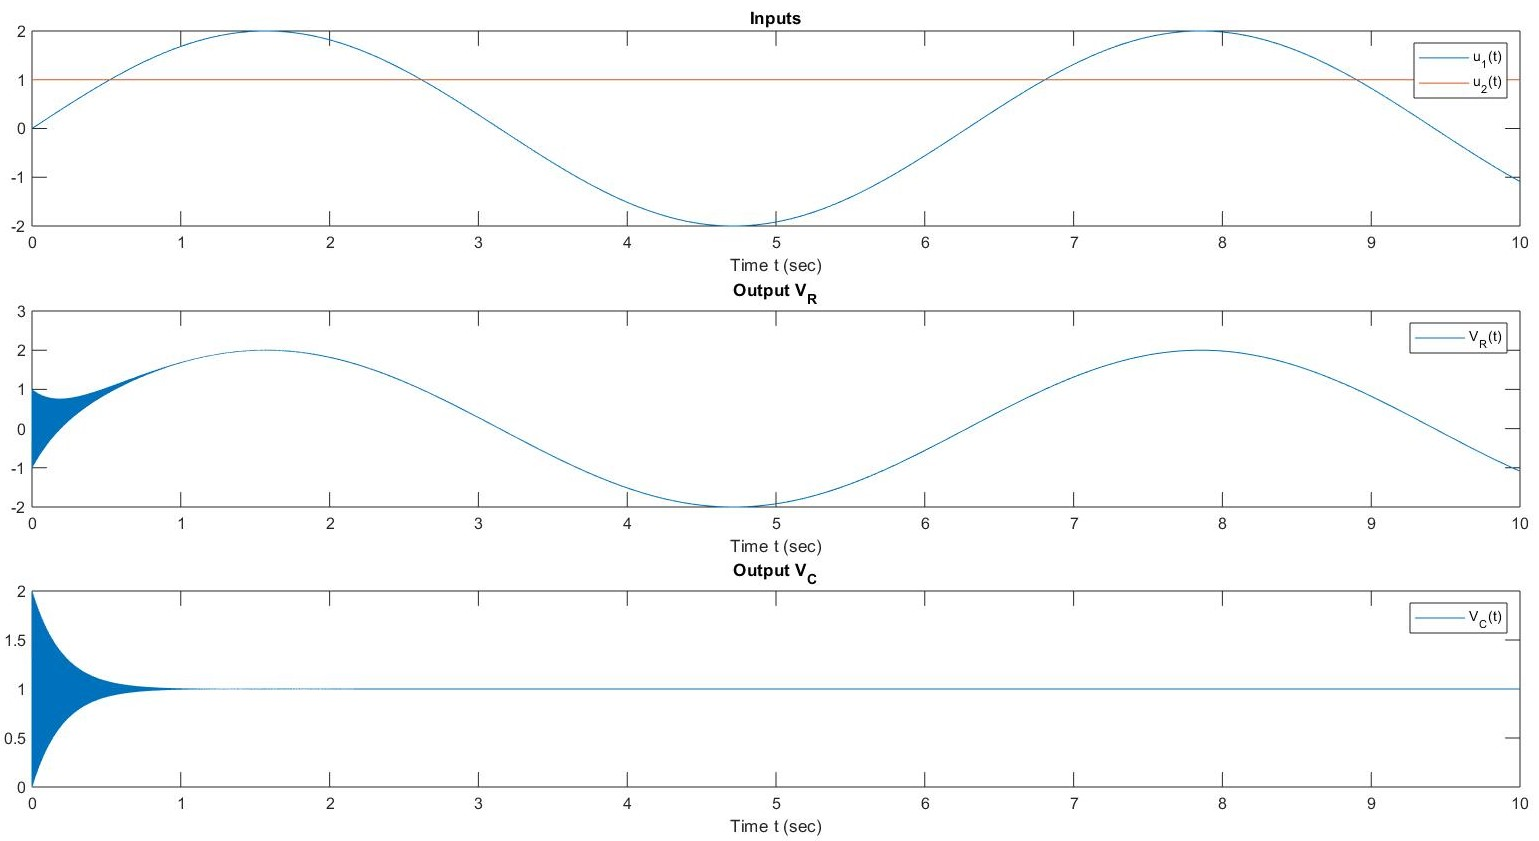
\includegraphics[width=\linewidth]{sys2_inp_out.jpg}
\centerline{Σχήμα 6: Είσοδοι - Έξοδοι Συστήματος}
\newline
\newline
\\
Οι γραφικές παραστάσεις των εισόδων και εξόδων του συστήματος, όταν εμφανίζονται σφάλματα-θόρυβος κατά τη μέτρηση (τυχαιές τιμές μεγαλύτερης τάξης μεγέθους σε εκατό τυχαίες θέσεις του κάθε πίνακα μετρήσεων $V_{R},V_{C}$) για χρόνο από $t=0$  μέχρι $t=10 sec$ με βήμα $0,000001$ φαίνονται στο Σχήμα 7.
\\ \\
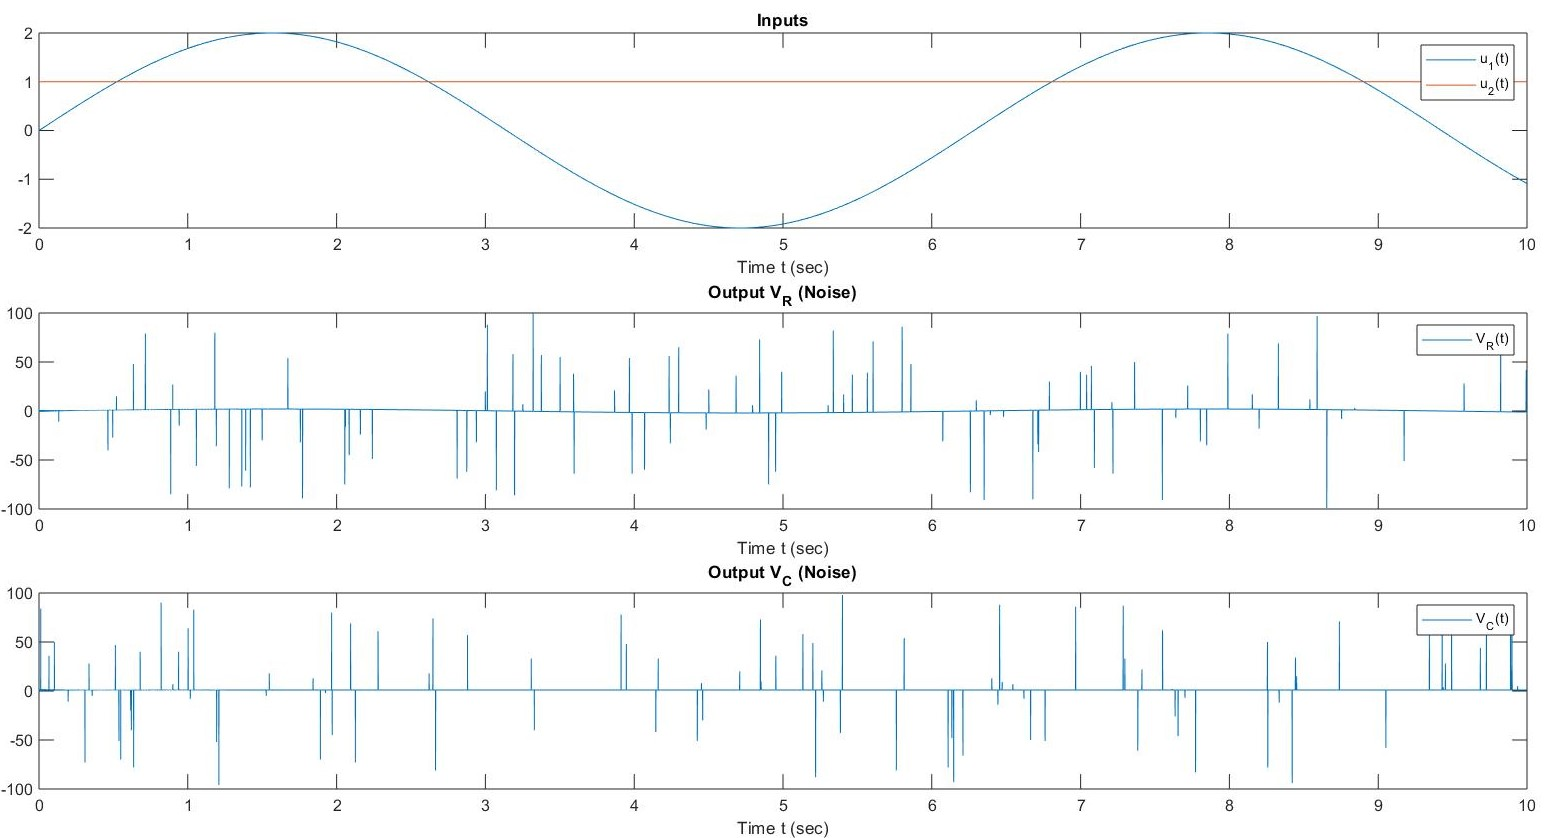
\includegraphics[width=\linewidth]{sys2_inp_falseout.jpg}
\centerline{Σχήμα 7: Είσοδοι - Έξοδοι Συστήματος με σφάλμα}
\newline
\newline
\\
Στο αρχείο $leastSquares.m$ υλοποιείται η μέθοδος ελαχίστων τετραγώνων όπως αναφέρθηκε στη θεωρητική ανάλυση του Θέματος 1, ενώ για τα διανύσματα οπισθοδρόμησης καλούνται οι συναρτήσεις $regressionVectorVr$ και $regressionVectorVc$. Για την εύρεση των $\theta_{0R}$ και $\theta_{0C}$ από την επίλυση των γραμμικών συστημάτων που προέκυψαν στο τέλος της μεθόδου, χρησιμοποιήθηκε η συνάρτηση $linsolve$ του $Matlab$.
\\ \\
Τέλος, στα αρχεία $regressionVectorVr.m$ και $regressionVectorVc.m$ παράγονται τα διανύσματα οπισθοδρόμησης. Συγκεκριμένα, αυτό επιτυγχάνεται, αναλυτικότερα, ως εξής.\\\\
Γράφουμε το διάνυσμα οπισθοδρόμησης $\zeta_{R}(s)$ στο πεδίο $Laplace$ ως
\\
$\zeta_{R}(s)=
\begin{bmatrix}
		\zeta_{1R}(s) & \zeta_{2R}(s) & \zeta_{3R}(s)  &  \zeta_{4R}(s)  &  \zeta_{5R}(s)  &  \zeta_{6R}(s)
\end{bmatrix}^{T}$ \quad άρα
\newline
\newline
$\zeta_{1R}(s)=-\frac{sV_{R}(s)}{s^2+\lambda_{1}s+\lambda_{2}} \Rightarrow \left( s^2+\lambda_{1}s+\lambda_{2} \right)\zeta_{1R}(s) = -sV_{R}(s)\xRightarrow{I.L.T.}$
\newline
$ \frac{d^2\zeta_{1R}}{dt^2} +\lambda_{1}\frac{d\zeta_{1R}}{dt}+\lambda_{2}\zeta_{1R}=-\frac{dV_{R}}{dt} \Rightarrow \ddot{\zeta_{1R}}+ \lambda_{1}\dot{\zeta_{1R}}+\lambda_{2}\zeta_{1R}=-\dot{V_{R}}$
\newline
\newline
\newline
$\zeta_{2R}(s)=-\frac{V_{R}(s)}{s^2+\lambda_{1}s+\lambda_{2}} \Rightarrow \left( s^2+\lambda_{1}s+\lambda_{2} \right)\zeta_{2R}(s) = -V_{R}(s)\xRightarrow{I.L.T.}$
\newline
$ \frac{d^2\zeta_{2R}}{dt^2} +\lambda_{1}\frac{d\zeta_{2R}}{dt}+\lambda_{2}\zeta_{2R}=-V_{R} \Rightarrow \ddot{\zeta_{2R}} +\lambda_{1}\dot{\zeta_{2R}}+\lambda_{2}\zeta_{2R}=-V_{R}$
\newline
\newline
\newline
$\zeta_{3R}(s)=\frac{U_{1}(s)}{s^2+\lambda_{1}s+\lambda_{2}} \Rightarrow \left( s^2+\lambda_{1}s+\lambda_{2} \right)\zeta_{3R}(s) = U_{1}(s)\xRightarrow{I.L.T.}$
\newline
$ \frac{d^2\zeta_{3R}}{dt^2} +\lambda_{1}\frac{d\zeta_{3R}}{dt}+\lambda_{2}\zeta_{3R}=u_{1} \Rightarrow \ddot{\zeta_{3R}} +\lambda_{1}\dot{\zeta_{3R}}+\lambda_{2}\zeta_{3R}=u_{1}$
\newline
\newline
$\zeta_{4R}(s)=\frac{U_{2}(s)}{s^2+\lambda_{1}s+\lambda_{2}} \Rightarrow \left( s^2+\lambda_{1}s+\lambda_{2} \right)\zeta_{4R}(s) = U_{2}(s)\xRightarrow{I.L.T.}$
\newline
$ \frac{d^2\zeta_{4R}}{dt^2} +\lambda_{1}\frac{d\zeta_{3R}}{dt}+\lambda_{2}\zeta_{3R}=u_{2} \Rightarrow \ddot{\zeta_{4R}} +\lambda_{1}\dot{\zeta_{3R}}+\lambda_{2}\zeta_{3R}=u_{2}$
\newline
\newline
$\zeta_{5R}(s)=\frac{s^{2}U_{1}(s)}{s^2+\lambda_{1}s+\lambda_{2}} \Rightarrow \left( s^2+\lambda_{1}s+\lambda_{2} \right)\zeta_{5R}(s) = s^{2}U_{1}(s)
\xRightarrow{I.L.T.}$
\newline
$ \frac{d^2\zeta_{5R}}{dt^2} +\lambda_{1}\frac{d\zeta_{5R}}{dt}+\lambda_{2}\zeta_{5R}=\ddot{u_{1}} \Rightarrow \ddot{\zeta_{5R}} +\lambda_{1}\dot{\zeta_{5R}}+\lambda_{2}\zeta_{5R}=\ddot{u_{1}}$
\newline
\newline
$\zeta_{6R}(s)=\frac{s^{2}U_{2}(s)}{s^2+\lambda_{1}s+\lambda_{2}} \Rightarrow \left( s^2+\lambda_{1}s+\lambda_{2} \right)\zeta_{6R}(s) = s^{2}U_{2}(s)
\xRightarrow{I.L.T.}$
\newline
$ \frac{d^2\zeta_{6R}}{dt^2} +\lambda_{1}\frac{d\zeta_{6R}}{dt}+\lambda_{2}\zeta_{6R}=\ddot{u_{2}} \Rightarrow \ddot{\zeta_{6R}} +\lambda_{1}\dot{\zeta_{6R}}+\lambda_{2}\zeta_{6R}=\ddot{u_{2}}$
\newline
\newline
Αντίστοιχα για το $V_{C}$ γράφουμε το διάνυσμα οπισθοδρόμησης $\zeta_{C}(s)$ στο πεδίο $Laplace$ ως
\\
$\zeta_{C}(s)=
\begin{bmatrix}
		\zeta_{1C}(s) & \zeta_{2C}(s) & \zeta_{3C}(s)  &  \zeta_{4C}(s) &  \zeta_{5C}(s) &  \zeta_{6C}(s)
\end{bmatrix}^{T}$ \quad άρα
\newline
\newline
$\zeta_{1C}(s)=-\frac{sV_{C}(s)}{s^2+\lambda_{1}s+\lambda_{2}} \Rightarrow \left( s^2+\lambda_{1}s+\lambda_{2} \right)\zeta_{1C}(s) = -sV_{C}(s)\xRightarrow{I.L.T.}$
\newline
$ \frac{d^2\zeta_{1C}}{dt^2} +\lambda_{1}\frac{d\zeta_{1C}}{dt}+\lambda_{2}\zeta_{1C}=-\frac{dV_{C}}{dt} \Rightarrow \ddot{\zeta_{1C}}+ \lambda_{1}\dot{\zeta_{1C}}+\lambda_{2}\zeta_{1C}=-\dot{V_{C}}$
\newline
\newline
$\zeta_{2C}(s)=-\frac{V_{C}(s)}{s^2+\lambda_{1}s+\lambda_{2}} \Rightarrow \left( s^2+\lambda_{1}s+\lambda_{2} \right)\zeta_{2C}(s) = -V_{C}(s)\xRightarrow{I.L.T.}$
\newline
$ \frac{d^2\zeta_{2C}}{dt^2} +\lambda_{1}\frac{d\zeta_{2C}}{dt}+\lambda_{2}\zeta_{2C}=-V_{C} \Rightarrow \ddot{\zeta_{2C}} +\lambda_{1}\dot{\zeta_{2C}}+\lambda_{2}\zeta_{2C}=-V_{C}$
\newline
\newline
$\zeta_{3C}(s)=\frac{U_{1}(s)}{s^2+\lambda_{1}s+\lambda_{2}} \Rightarrow \left( s^2+\lambda_{1}s+\lambda_{2} \right)\zeta_{3C}(s) = U_{1}(s)\xRightarrow{I.L.T.}$
\newline
$ \frac{d^2\zeta_{3C}}{dt^2} +\lambda_{1}\frac{d\zeta_{3C}}{dt}+\lambda_{2}\zeta_{3C}=u_{1} \Rightarrow \ddot{\zeta_{3C}} +\lambda_{1}\dot{\zeta_{3C}}+\lambda_{2}\zeta_{3C}=u_{1}$
\newline
\newline
$\zeta_{4C}(s)=\frac{U_{2}(s)}{s^2+\lambda_{1}s+\lambda_{2}} \Rightarrow \left( s^2+\lambda_{1}s+\lambda_{2} \right)\zeta_{4C}(s) = U_{2}(s)\xRightarrow{I.L.T.}$
\newline
$ \frac{d^2\zeta_{4C}}{dt^2} +\lambda_{1}\frac{d\zeta_{4C}}{dt}+\lambda_{2}\zeta_{4C}=u_{2} \Rightarrow \ddot{\zeta_{4C}} +\lambda_{1}\dot{\zeta_{4C}}+\lambda_{2}\zeta_{4C}=u_{2}$
\newline
\newline
$\zeta_{5C}(s)=\frac{sU_{1}(s)}{s^2+\lambda_{1}s+\lambda_{2}} \Rightarrow \left( s^2+\lambda_{1}s+\lambda_{2} \right)\zeta_{5C}(s) = sU_{1}(s)
\xRightarrow{I.L.T.}$
\newline
$ \frac{d^2\zeta_{5C}}{dt^2} +\lambda_{1}\frac{d\zeta_{5C}}{dt}+\lambda_{2}\zeta_{5C}=\dot{u_{1}} \Rightarrow \ddot{\zeta_{5C}} +\lambda_{1}\dot{\zeta_{5C}}+\lambda_{2}\zeta_{5C}=\dot{u_{1}}$
\newline
\newline
$\zeta_{6C}(s)=\frac{sU_{2}(s)}{s^2+\lambda_{1}s+\lambda_{2}} \Rightarrow \left( s^2+\lambda_{1}s+\lambda_{2} \right)\zeta_{6C}(s) = sU_{2}(s)
\xRightarrow{I.L.T.}$
\newline
$ \frac{d^2\zeta_{6C}}{dt^2} +\lambda_{1}\frac{d\zeta_{6C}}{dt}+\lambda_{2}\zeta_{6C}=\dot{u_{2}} \Rightarrow \ddot{\zeta_{6C}} +\lambda_{1}\dot{\zeta_{6C}}+\lambda_{2}\zeta_{6C}=\dot{u_{2}}$
\newline
\newline
Με τη βοήθεια της συνάρτησης $lsim$ του $Matlab$ επιλύουμε τις παραπάνω διαφορικές εξισώσεις με μηδενικές αρχικές συνθήκες και βρίσκουμε αριθμητικά στο χρόνο τις $\zeta_{1R},\zeta_{2R},\zeta_{3R},\zeta_{4R},\zeta_{5R},\zeta_{6R}$ και $\zeta_{1C},\zeta_{2C},\zeta_{3C},\zeta_{4C},\zeta_{5C},\zeta_{6C}$ με τη μορφή πίνακα.
\subsection{Έλεγχος Σφαλμάτων}
Προκειμένου να ελέγξουμε τις εκτίμησεις μας για τις ζητούμενες παραμέτρους $\frac{1}{RC}$ και $\frac{1}{LC}$ θεωρούμε τα σφάλματα  $e_{R}$ , $e_{C}$
\[e_{R}=|V_{R} - \widetilde{V_{R}}|\]
\[e_{C}=|V_{C} - \widetilde{V_{C}}| \]
\\
που μας δείχνουν πόσο διαφέρουν, κατά απολύτη τιμή,  οι πραγματικές έξοδοι του συστήματος (όπως δειγματοληπτούνται από το αρχείο $v.p$) σε σχέση με τις εξόδους όπως προκύπτουν από την επίλυση της διαφορικής εξίσωσης $(10)$.
\\ \\
Με $\widetilde{V_{R}}$,$\widetilde{V_{C}}$ συμβολίζονται οι εκτιμήσεις των $V_{R}$,$V_{C}$ αντίστοιχα, όπως προκύπτουν από την επίλυση της διαφορικής εξίσωσης (10) για τις τιμές των παραμέτρων μου εκτιμήσαμε.
\\ \\
Οι γραφικές παραστάσεις των σφαλμάτων φαίνονται, αντίστοιχα, στο Σχήμα 8.
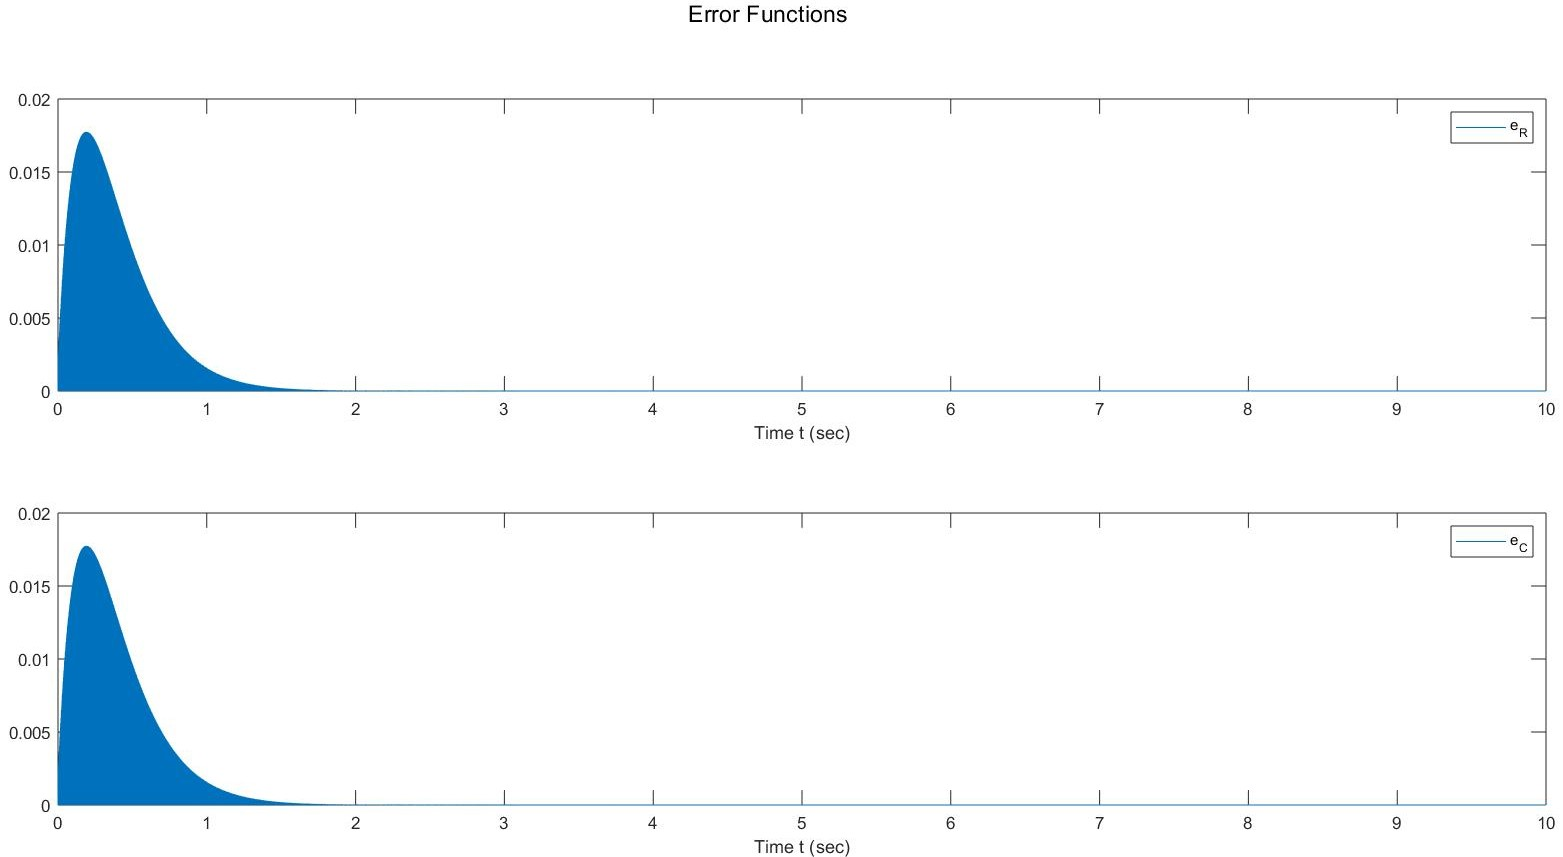
\includegraphics[width=\linewidth]{sys2_error.jpg}
\\ \\
\centerline{Σχήμα 8}
\centerline{Γραφικές παραστάσεις σφαλμάτων $e_{R}$ και $e_{C}$}
\\ \\ \\
Βλέπουμε, λοιπόν, ότι το σφάλμα είναι πολύ μικρό και επομένως οι τιμές των $RC$ και $LC$ προσεγγίζουν αρκετά καλά την πραγματικότητα.
\\
Αντίστοιχα στην περίπτωση που υπάρχουν σφάλματα στις μετρήσεις των εξόδων, τα παραπάνω σφάλματα έχουν τις γραφικές παραστάσεις του Σχήματος 9.
\\ \\
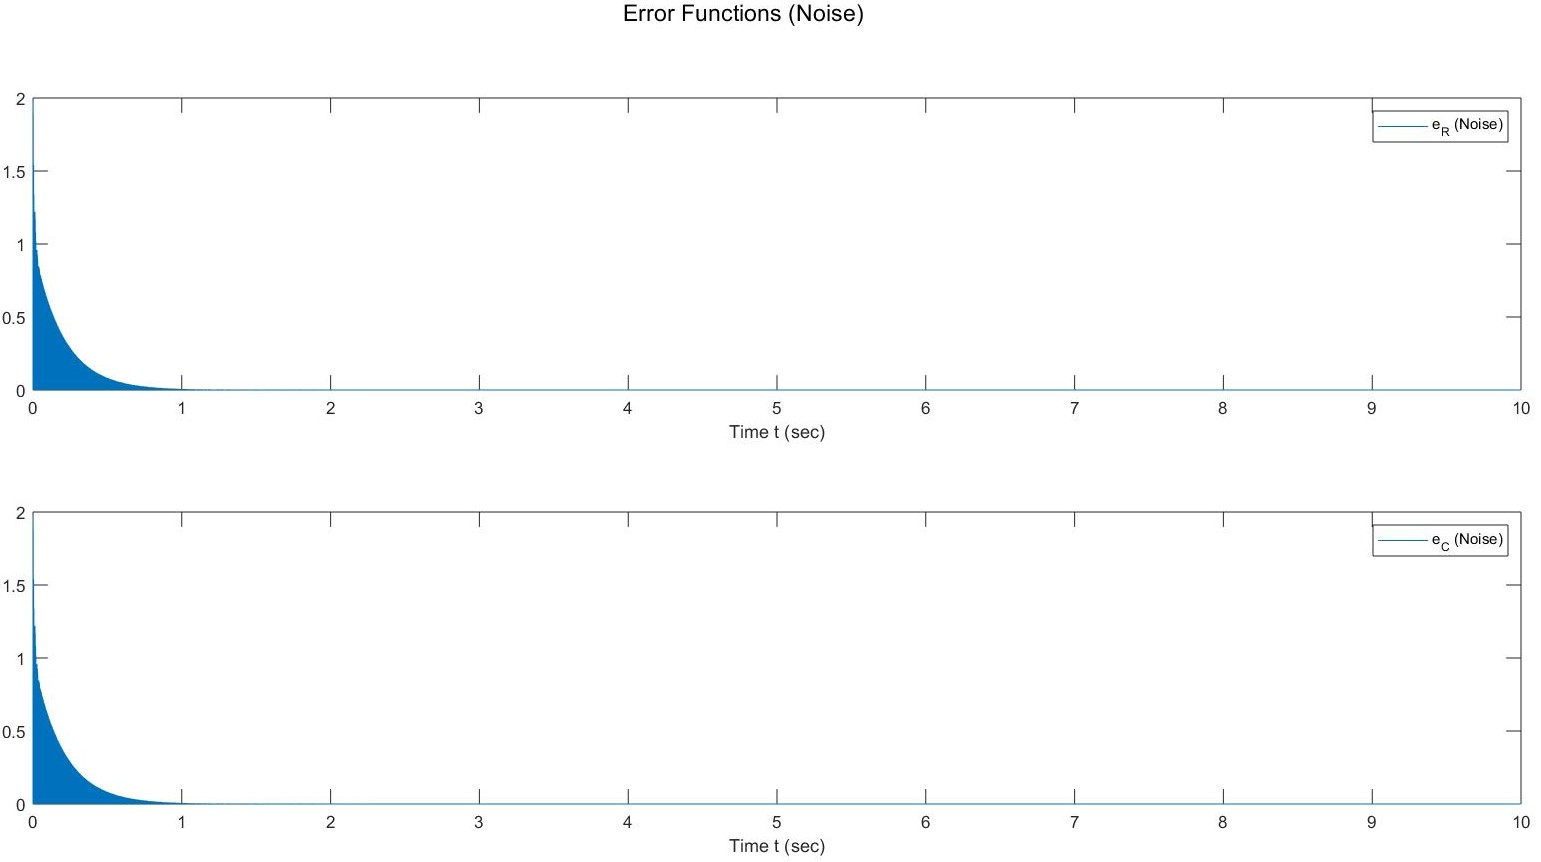
\includegraphics[width=\linewidth]{sys2_error_noise.jpg}
\\ \\
\centerline{Σχήμα 9}
\centerline{Γραφικές παραστάσεις σφαλμάτων $e_{R}$ και $e_{C}$ με την ύπαρξη θορύβου}
\\ \\ \\
Από τα σχήματα φαίνεται ότι το σφάλμα είναι σημαντικά υψηλότερο όταν εμφανίζεται θόρυβος, κάτι που ήταν αναμενώμενο από τις τιμές των παραμέτρων που εκτιμήθηκαν στο τέλος της ενότητας 2.1.
\end{document}